\documentclass[11pt,a4paper]{article}
\usepackage[margin=2.5cm]{geometry}
\usepackage{graphicx}
\usepackage{enumitem}
\usepackage[svgnames]{xcolor}
\usepackage[most]{tcolorbox}
\usepackage[hidelinks]{hyperref} % o usar colorlinks como se explicó antes
\usepackage{listings}
\usepackage[spanish]{babel}
\usepackage{changepage}
\usepackage{enumitem}

\lstset{
	language=C, % Lenguaje: C
	basicstyle=\ttfamily\small, % Fuente monoespaciada, tamaño pequeño
	keywordstyle=\color{Blue}\bfseries, % Palabras clave en azul y negrita
	stringstyle=\color{Red}, % Cadenas en rojo
	commentstyle=\color{Green}, % Comentarios en verde
	numbers=left, % Numeración de líneas a la izquierda
	numberstyle=\tiny\color{Gray}, % Estilo de números de línea
	stepnumber=1, % Numerar cada línea
	numbersep=5pt, % Distancia de números al código
	showspaces=false, % No mostrar espacios
	showstringspaces=false, % No marcar espacios en cadenas
	frame=single, % Marco alrededor del código
	tabsize=4, % Tamaño de tabulación
	breaklines=true, % Romper líneas largas
	breakatwhitespace=true, % Romper solo en espacios
}

\begin{document}
	\begin{titlepage}
		\begin{center}
			\begin{figure}
				\centering
				
\includegraphics[scale=0.2]{US-marca-principal.png}
			\end{figure}
			{\large \textbf{Escuela Técnica Superior de Ingeniería Informática}}
			\vspace{2mm}\\
			{Ingeniería Informática. Ingeniería de Computadores.}
			\vspace{60mm}\\
			\begin{center}
				{\huge \textbf{MEMORIA PRÁCTICA I}}\\[2mm]
				{Asignatura: Sistemas Empotrados y de Tiempo Real I}\\
				{Profesor: Gabriel Jiménez Moreno}
			\end{center}
			\vfill
			{Alumno: Álvaro José Gullón Vega}
		\end{center}
	\end{titlepage}
	\pagebreak
	\tableofcontents
	\pagebreak
	
	\section{Objetivos}
	\large{
		En esta primera práctica distinguimos dos objetivos:
		
	\subsection{Académico}
		Como objetivo académico, la práctica nos introduce al sector de la programación de microcontroladores a través de la instalación y posterior uso de el entorno de desarrollo STM32CubeIDE, que se puede complementar con el simulador QEMU para realizar proyectos en los que no haya posibilidad de adquirir el hardware a usar.
	\subsection{Práctico}
		En cuanto al objetivo práctico, la práctica se fundamenta en dar una explicación sobre el entorno para ir familiarizándonos con él junto a unas instrucciones detalladas para la correcta instalación de este junto al simulador a usar, incluyendo nociones básicas sobre configuraciones del proyecto y cómo debemos ejecutarlo.
	}
	
	\section{Introducción}
	\large{
		En esta práctica por motivos de calendario, se ha hecho de forma no presencial sin ninguna explicación de profesor (quitando el documento proporcionado). Como hemos mencionado anteriormente, esta práctica trata sobre la introducción al sistema de desarrollo STM32CubeIDE, que será el entorno de desarrollo que usaremos durante todo el curso, junto a la instalación de un simulador llamado QEMU para la implementación de aplicaciones cuando no tenemos recursos hardware disponibles.\\

		La placa con la que vamos a probar el sistema es la STM32 Cortex M0, pese a que en el resto de las prácticas vamos a usar una STM32 Cortex M4 con gran cantidad de periféricos. Como parte esencial de esta y de todas las prácticas, usaremos STM32CubeIDE, que está basado en Eclipse, para programar nuestros microcontroladores.\\
		
		Vemos diferenciadas varias fases o etapas a lo largo de la práctica que nos indican el desarrollo que debemos llevar. En la primera fase tenemos que llevar a cabo la instalación del entorno de desarrollo STM32CubeIDE. Es una mezcla de varias herramientas de desarrollo que han ido evolucionando e integrándose
		en un solo entorno, SW4STM32 + Atollic TrueStudio + STM32CubeMX, los primeros eran entornos de desarrollo IDE
		y el último un generador automático de código de configuración de los microcontroladores STM. Particularmente, he usado la última versión disponible en la página web del fabricante, la versión 1.17.0.\\

		Tras esto, nos disponemos a comenzar con la creación del proyecto y posteriormente las fases contenidas en la práctica recogidas en el documento a descargar de la Enseñanza Virtual.
	}
	
	\section{Desarrollo de la práctica}
	\subsection{Fase 1: Instalación del sistema de desarrollo STM32CubeIDE y del simulador QEMU}
	En esta primera fase, el objetivo es la correcta instalación del entorno de desarollo. En primer lugar, debemos visitar la página web de STMicroelectronics y descargarnos el software, en mi caso he descargado la versión 1.17.0. La instalación de este es muy sencillo, pues basta con abrir el ejecutable descargado y darle a siguiente hasta acabar el proceso.\\
	
	Una vez instalado, lo abrimos y procedemos a instalar el simulador QEMU para, valga la redundancia, simular el hardware de esta práctica. Para instalarlo, nos vamos al menú superior y pulsamos en: \textit{Help $\rightarrow$ Eclipse Marketplace} y dentro de esta venta buscamos \textit{GNU MCU Eclipse} y el resultado es lo que debemos instalar. Por último, debemos ir al enlace de GitHub del enunciado de la práctica donde están los paquete de simulación para los ARM Cortex e instalarlos en nuestro equipo. Con estos pasos ya estaría todo preparado para programar.
	
	\subsection{Fase 2: Encender un LED}
	Tras proceder con la correcta instalación del entorno de desarrollo y los ajustes necesarios para el funcionamiento de este, se nos propone probar su funcionamiento desarrollando un simple programa que nos permite encender y apagar un LED de la placa que estamos usando para comprobar que todo funciona correctamente. En la guía nos indica cómo crear un proyecto para este caso y la placa que debemos usar, que se trata de la \textbf{NUCLEO-F103RB}. Es importante que cuando al crear el proyecto nos pregunte sobre si queremos inicializar los periféricos debemos decir que sí, de esta forma existe un determinado pin, como el del LED que queremos encender, se coloca por defecto como salida.\\
	
	Una vez creado el proyecto, disponemos de una funcionalidad que nos permite generar el código de configuración de nuestro microcontrolador en base a si están los valores por defecto o si hemos modificado elementos como el reloj o los GPIO. Es importante que si tenemos una configuración y por cualquier motivo hemos tenido que modificar por ejemplo la frecuencia del reloj, debemos volver a generar el código para que las modificaciones se vean efectuadas. Para esta fase, no vamos a modificar nada de la configuración inicial, por lo que pulsamos en \textit{Project $\rightarrow$ Generate Code} para generar nuestro fichero de configuración.\\
	
	Procedemos a escribir el código en el fichero \textit{main.c}. Debemos escribir el código entre los comentarios de \footnotesize\textcolor{DarkGreen}{{\textbf{/*USER CODE BEGIN… *//* USER CODE END … *}}} \large para evitar que, en caso de que se vuelva a hacer, cuando generemos el código de configuración de nuestro proyecto se pierda.\\
	
	La estructura es sencilla, primero los includes y luego el código. Entonces, arriba del main, en la sección de los includes debemos escribir lo siguiente:
	\begin{lstlisting}
	void SystemClock_Config(void); // sirve para inicializar el reloj
	static void MX_GPIO_Init(void); // sirve para inicializar los GPIO
	static void MX_USART2_UART_Init(void); // sirve para inicializar un puerto serie
	\end{lstlisting}
	\vspace{1em}
	
	Posterior a esto debemos ir a nuestra función main, donde se encuentra el while(1) tan importante y fundamental de los microcontroladores en el que debemos escribir nuestro código, pero antes debemos saber como se escribe y se lee un pin. Nosotros usaremos la librería HAL que nos proporcionan estas dos funciones:
	\begin{lstlisting}
	HAL_GPIO_WritePin(GPIOA, GPIO_PIN_5, 0); // pone a cero el LED
	HAL_GPIO_ReadPin(GPIOC, GPIO_PIN_13); // devuelve el valor del boton
	\end{lstlisting}
	\vspace{1em}
	
	En nuestro caso, si queremos que se encienda el LED en base a si pulsamos o no el botón debemos poner la siguiente línea dentro del while(1):
	\begin{lstlisting}
	HAL_GPIO_WritePin(LD2_GPIO_Port, LD2_Pin, HAL_GPIO_ReadPin(B1_GPIO_Port, B1_Pin));
	\end{lstlisting}
	\vspace{1em}
	
	Tras esto, podemos terminar de configurar el simulador QEMU para que funcione correctamente. Para ello, vamos a \textit{Window $\rightarrow$ Preferences} y aquí dentro indicamos la ruta de donde se encuentra la carpeta \textit{bin} de los archivos xPack que nos habíamos descargado previamente. Después de esto, el último paso es dirigirnos a \textit{Run $\rightarrow$ Debug Configuration} y configurar el depurador de nuestro proyecto. Una vez configurado correctamente, procedemos a darle \textit{Debug} y nos debería salir la siguiente imagen simulando a nuestra placa:
	
	\begin{figure}[h!]
		\centering
		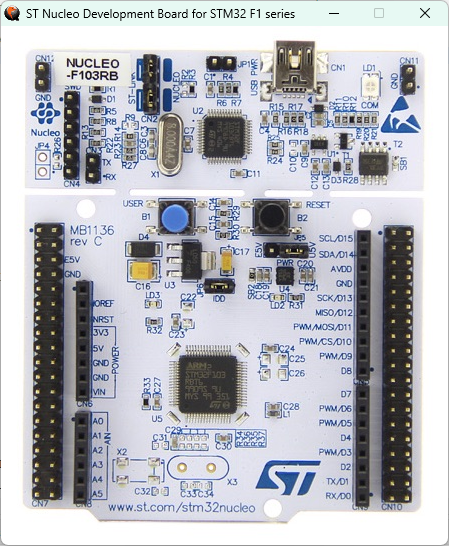
\includegraphics[width=0.6\textwidth]{placa-empty.png}
		\caption{Inicialización de la placa seleccionada.}
		\label{fig:placa-vacia}
	\end{figure}
	
	Si todo funciona como debe ser, si pulsamos el botón azul se debería encender el LED, tal y como lo hemos programado. El resultado sería el siguiente:
	
		\begin{figure}[h!]
		\centering
		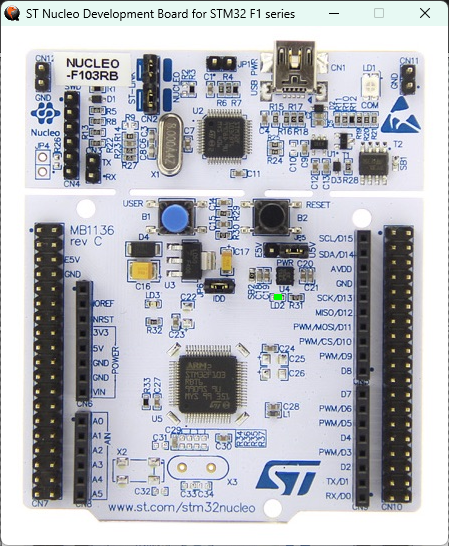
\includegraphics[width=0.6\textwidth]{placa-led.png}
		\caption{Resultado Fase 2.}
		\label{fig:placa-led}
	\end{figure}
	
	\subsection{Fase 3: Utilizar la interrupción de pulsar botón para cambiar el estado del LED}
	En esta fase lo que vamos a realizar es que el botón conmute el estado del LED, de forma que si este está apagado y pulsamos el botón se encienda y el caso contrario, que si está encendido y pulsamos el botón este se apague. Se podría hacer sin el uso de interrupciones, pero en este ocasión vamos a utilizarlas.\\
	
	Abrimos el fichero .io de nuestro proyecto para ver cómo están configurados los pines de nuestra placa y hacer modificaciones varias. Observamos que el pin PC13 está configurado como GPIO\_EXTI13. Seleccionamos la pestañana \textit{System view} y posteriormente seleccionamos GPIO. Si seleccionamos PA5 podemos ver las caracterícticas del pin:
	\begin{itemize}
		\item \textbf{GPIO Output Level:} valor inicial del pin, si es salida
		\item \textbf{GPIO Mode:} en caso de salida, si es Push Pull u Open Drain
		\item \textbf{GPIO Pull Up/Pull Down:} si se activa o no algunas de las resistencias internas del microcontrolador
		correspondientes a ese pin y conectadas a VCC o a GND.
		\item \textbf{Maximum output speed:} si la conmutación del pin en caso de que fuera de salida es rápida o lenta.
		\item \textbf{User label:}  es una etiqueta que se le asigna al pin y con la que podemos referirnos a él en nuestro código, se
		podría dejar en blanco y utilizar la denominación de los pines como vimos antes, o colocar cualquier nombre en la
		etiqueta.\\
	\end{itemize}
	
	Si seleccionamos PC13 podemos elegir además el modo de disparo de la interrupción (flanco de bajada, flanco de subida o ambos de la señal de entrada). Ajustado esto, procedemos a comprobar la configuración del controlador de interrupciones accediendo a las siguientes pestañas: \textit{System Core $\rightarrow$ NVIC $\rightarrow$ Code Generation}. No hace falta que ajustemos nada ya que tras haber generado el código está todo correctamente, por tanto, nos dirigimos al fichero \textbf{\textit{STM32F1xx\_it.c}} en el que tenemos todas las rutinas de interrupción principales. La interrupción por un pin externo se maneja en la función \textit{HAL\_GPIO\_EXTI\_IRQHandler()}, que accediendo a su declaración nos encontramos con el archivo en el que debemos colocar nuestro código en la función \textit{HAL\_GPIO\_EXTI\_Callback}. Dentro de esta función nos indica que no hay que modificarla ni tocar nada en ella, que debemos crear una igual en el fichero \textit{main.c}, pero tendríamos dos funciones que se llamen igual, ¿cómo sabemos a cuál salta cuando se llame? Muy sencillo. Existe una forma de declarar la función como \textit{\_\_weak}, que significa que si hay dos funciones que se denominan igual, el linker se decidirá por la que no es \textit{\_\_weak}.\\
	
	Entonces, debemos colocar en el fichero \textit{main.c} el nombre de esa función de callback:
	\begin{lstlisting}
		void HAL_GPIO_EXTI_Callback(uint16_t GPIO_Pin)
	\end{lstlisting}
	\vspace{1em}
	
	Debemos colocarlo entre algún BEGIN - END para evitar que se borre en la posibilidad de que se tenga que volver a usar la función de Generate Code. En nuestro caso lo hemos colocado entre estos BEGIN - END:
	\begin{lstlisting}
	/* USER CODE BEGIN 4 */
	void HAL_GPIO_EXTI_Callback(uint16_t GPIO_Pin)
	{
		static char estado=0;
		if (estado ==1)
		{
			HAL_GPIO_WritePin(LD2_GPIO_Port, LD2_Pin, GPIO_PIN_SET);
			estado=0;
		}
		else
		{
			HAL_GPIO_WritePin(LD2_GPIO_Port, LD2_Pin, GPIO_PIN_RESET);
			estado=1;
		}
	}
	/* USER CODE END 4 */
	\end{lstlisting}
	\vspace{1em}
	
	Junto a esto, debemos comentar la línea que pusimos en la fase pasada dentro del bucle while(1). Una vez completado esto podemos comprobar que funciona correctamente, por tanto, compilamos y depuramos como hemos hecho en la fase anterior.\\
	
	\begin{tcolorbox}[colback=gray!10, colframe=gray!60, title=Nota informativa]
		Hay una pregunta sobre por qué la variable estado se declara como \textit{static} que la he respondido en la Sección~\ref{sec:contestacion1}.
	\end{tcolorbox}
	
	\subsection{Fase 4: Hacer que le LED se encienda y apague a un determinado ritmo}
	Para hacer intermitencia con el LED con un periodo bastante exacto vamos a utilizar el timer del sistema Systick, que es común a todos los Cortex M independientemente del fabricante del chip. El Systick es un temporizador de 24 bits de cuenta descendente que produce una interrupción y lo recarga del contador cuando el registro interno llega a cero desde el valor de recarga inicial.\\
	
	Para realizar esta fase, debemos volver al generador de código y seleccionamos la pestaña \textit{Clock Configuration} para configurar y ver al estructura de los diferentes relojes. El Systick, con una entrada de 64 MHz y un contador de 24 bits, permite una interrupción periódica máxima de 0,262 segundos (con valor de recarga 0xFFFFFF, es decir, poniendo todos sus 24 bits a 1). Este valor se configura con el siguiente código que debemos poner antes del while(1) tratándolo como inicializamos un periférico:
	\begin{lstlisting}
		HAL_SYSTICK_Config(0xffffff);
	\end{lstlisting}
	\vspace{1em}
	
	Para que el LED conmute, debemos escribir lo siguiente en el fichero \textit{stm32f1xx\_it.c} en la función de interrupción:
	\begin{lstlisting}
	/* USER CODE BEGIN SysTick_IRQn 0 */
	static char estado=0;
	if (estado ==1)
	{
		HAL_GPIO_WritePin(LD2_GPIO_Port, LD2_Pin, GPIO_PIN_SET);
		estado=0;
	}
	else
	{
		HAL_GPIO_WritePin(LD2_GPIO_Port, LD2_Pin, GPIO_PIN_RESET);
		estado=1;
	}
	/* USER CODE END SysTick_IRQn 0 */
	\end{lstlisting}
	\vspace{1em}
	
	Y con esto estaría todo funcionando correctamente.
	
	\begin{tcolorbox}[colback=gray!10, colframe=gray!60, title=Nota informativa]
		Preguntas sobre si debemos comentar el código anterior y cómo podemos hacer que el LED parpadee más lento resueltas en la Sección~\ref{sec:contestacion2}.
	\end{tcolorbox}
	
	\section{Contestación de preguntas}
	
	\label{sec:contestacion1}
	\begin{description}
		\item[\textbf{Fase 3 - ¿Por qué la variable \texttt{estado} está declarada como \texttt{static}?}]
		\hfill\\
		La palabra clave \texttt{static} indica que la variable conserva su valor entre ejecuciones del bucle, como si se inicializara una sola vez. Esto es necesario porque, si se declarara como una variable local normal, se reinicializaría en cada iteración y no podría mantener el estado anterior.
	\end{description}
	
	\label{sec:contestacion2}
	\begin{description}[style=nextline]
		\item[\textbf{Fase 4 - ¿Es necesario que comentemos el código anterior que controla el Led con el botón azul?}]
		No, no es necesario comentar el código anterior, puesto que el uso del botón en este caso es nulo y no afecta a la intermitencia del LED.
		
		\item[\textbf{Fase 4 - ¿Y si quisiéramos que parpadeara más lento el LED, por ejemplo 16 veces más lento, sin cambiar nada del código?}]
		Tendríamos que cambiar la frecuencia del reloj HCL. Cambiaríamos en el generador de código el pre-escalador AHB a /16, eso pone el HCLK a 4Mhz, generar de nuevo el código, compilar y simular.
	\end{description}
	
	\begin{description}[style=nextline]
		\item[\textbf{Pregunta 1 - Buscar en la Wikipedia que es el Qemu y hacer un resumen en cinco líneas reflexionando sobre qué es lo que hemos montado en esta práctica.}]
		No, no es necesario comentar el código anterior, puesto que el uso del botón en este caso es nulo y no afecta a la intermitencia del LED.\\
		
		\item[\textbf{Pregunta 2 - ¿Qué podríamos haber hecho en nuestro código para que el diodo parpadeara 16 veces más lento que al principio de la fase 4 sin tocar para nada la configuración del reloj del sistema?}]
		Debemos modificar el código escrito en el archivo \textit{stm32f1xx.it.c} al siguiente:
		\begin{lstlisting}
		/* USER CODE BEGIN SysTick_IRQn 0*/
		static char estado = 0;
		if (estado == 0) {
			HAL_GPIO_WritePin(LD2_GPIO_Port, LD2_Pin, GPIO_PIN_SET);
			estado = estado + 1;
		} else if (estado == 16) {
			HAL_GPIO_WritePin(LD2_GPIO_Port, LD2_PIN, GPIO_PIN_RESET);
		} else if (estado == 32) {
			estado = 0;
		} else {
			estado = estado + 1;
		}
		/* USER CODE END SysTick_IRQn 0*/
		\end{lstlisting}
		\vspace{1em}
		
		El LED cambia de estado solamente cuando la variable \textit{estado} es igual a 0 o 16. Luego de alcanzar \textit{estado == 32}, este vuelve a 0 reiniciando el ciclo. Esto significa que el LED cambia de estado cada 16 interrupciones de SysTick.\\
		
		\item[\textbf{Pregunta 3 - La intermitencia del LED se realiza con precisión, pero con valores un poco al azar. Calcule con los parámetros que se han usado cuánto tiempo está encendido el LED y cuánto tiempo está apagado. Y ahora, al contrario, busca una combinación de la configuración del reloj HCLK (con el CubeMX) y el valor de recarga del SYSTICK que haga que el LED esté con una intermitencia de 0,5 segundos encendido y 0,5 segundos apagado. En la figura del esquema del timer Systick hay una expresión en la que se muestra el cálculo del periodo de interrupción}]
		Como el registro del contador posee 24 bits, tenemos \( 2^{24} \) posibles valores. La frecuencia más baja que podemos generar será \( \frac{2^{24}}{6400000} \), ya que la frecuencia del reloj es de 64 MHz. Calculando:
		
		\[
		\frac{2^{24}}{6400000} = 0.262144 \, \text{segundos estará el LED encendido/apagado}
		\]\\
		
		Para el caso contrario, accedemos al \textit{Clock Configuration} y cambiamos el valor del AHB Prescaler para dividir la frecuencia del reloj HCLK.
		Probando valores, obtenemos que con una frecuencia de 32MHz podemos tener los 0,5 segundos de encendido y apagado.
		
	\end{description}
	

	\section{Conclusiones}
	Tras haber realizado la práctica he aprendido a como simular una placa y he aprendido a instalar, tener conocimientes básicos sobre cómo usar y configurar el IDE y una introducción a la programación de los sistemas empotrados. En mi caso, sí he conseguido los objetivos tras la realización de la práctica y las fases propuestas por el profesorado. He tenido que indagar más en la parte de las preguntas puesto que al ser la primera práctica y no haber tenido contacto con este entorno ni profundizar tanto en aspectos de frecuencia de reloj, pines, interrupciones, etc... me ha costado más, pero he acabado con más conocimientos sobre ello que al fin y al cabo es lo importante.
\end{document}